\documentclass[11pt]{article}
\usepackage{listings}
\usepackage{tikz}
%\usepackage{algorithm2e}
\usetikzlibrary{arrows,automata,shapes}
\tikzstyle{block} = [rectangle, draw, fill=blue!20, 
    text width=5em, text centered, rounded corners, minimum height=2em]
\tikzstyle{bt} = [rectangle, draw, fill=blue!20, 
    text width=1em, text centered, rounded corners, minimum height=2em]

\lstset{ %
language=Java,
basicstyle=\ttfamily\scriptsize,commentstyle=\scriptsize\itshape,showstringspaces=false,breaklines=true}

\newtheorem{defn}{Definition}
\newtheorem{crit}{Criterion}

\newcommand{\handout}[5]{
  \noindent
  \begin{center}
  \framebox{
    \vbox{
      \hbox to 5.78in { {\bf Software Testing, Quality Assurance and Maintenance } \hfill #2 }
      \vspace{4mm}
      \hbox to 5.78in { {\Large \hfill #5  \hfill} }
      \vspace{2mm}
      \hbox to 5.78in { {\em #3 \hfill #4} }
    }
  }
  \end{center}
  \vspace*{4mm}
}

\newcommand{\lecture}[4]{\handout{#1}{#2}{#3}{#4}{Lecture #1}}
\topmargin 0pt
\advance \topmargin by -\headheight
\advance \topmargin by -\headsep
\textheight 8.9in
\oddsidemargin 0pt
\evensidemargin \oddsidemargin
\marginparwidth 0.5in
\textwidth 6.5in

\parindent 0in
\parskip 1.5ex
%\renewcommand{\baselinestretch}{1.25}

\begin{document}

\lecture{2 --- January 7/9, 2017}{Winter 2019}{Patrick Lam}{version 1}

\section*{Faults, Errors, and Failures}
For this course, we are going to define the following terminology.

\begin{itemize}
\item {\bf Fault} (also known as a bug): A static defect in software---incorrect lines of code.
\item {\bf Error}: An incorrect internal state---not necessarily observed yet.
\item {\bf Failure}: External, incorrect behaviour with respect to the expected behaviour---must be visible (e.g. EPIC FAIL).
\end{itemize}

These terms are not used consistently in the literature. Don't get stuck on memorizing them.

\paragraph{Motivating Example.} Here's a train-tracks analogy.
\begin{center}
  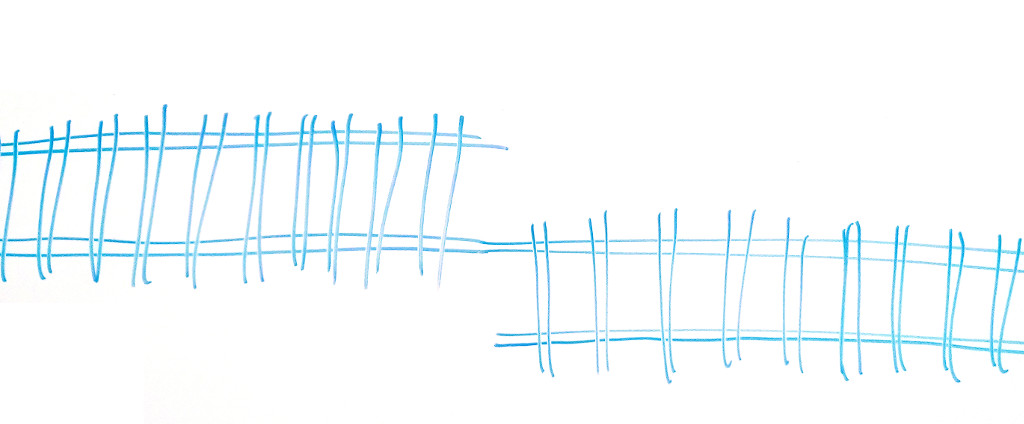
\includegraphics[width=.7\textwidth]{L02/001_fault_error_or_failure}\\
  (all railroad pictures inspired by: Bernd Bruegge \& Allen H. Dutoit, \emph{Object Oriented Software Engineering: Using UML, Patterns and Java}.)
\end{center}
Is it a failure? An error? A fault? Clearly, it's not right. But no
failure has occurred yet; there is no behaviour. I'd also say that
nothing analogous to execution has occurred yet either.  If there was
a train on the tracks, pre-derailment, then there would be an error.
That picture most closely corresponds to a fault.

\newpage Perhaps it was caused by mechanical stresses.
\begin{center}
  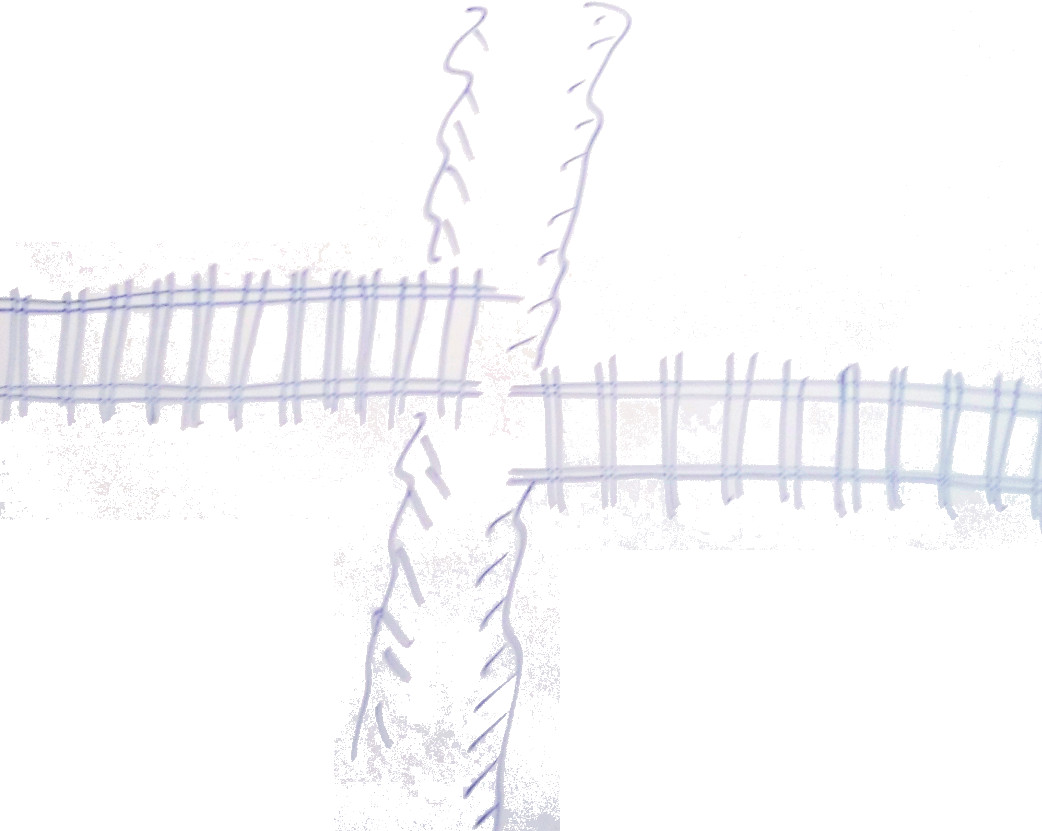
\includegraphics[width=.7\textwidth]{L02/002_mechanical_fault}
\end{center}
Or maybe it was caused by poor design.

\paragraph{Software-related Example.}
Let's get back to software and consider this code:
\begin{lstlisting}
  public static numZero(int[] x) {
    // effects: if x is null, throw NullPointerException
    //          otherwise, return number of occurrences of 0 in x.
    int count = 0;
    for (int i = 1; i < x.length; i++) {
      // program point (*)
      if (x[i] == 0) count++; 
    } 
    return count;
  }
\end{lstlisting}
As we saw, it has a fault (independent of whether it is executed
or not): it's supposed to return the number of 0s, but it doesn't
always do so.
We define the state for this method to be the variables {\tt x},
{\tt i}, {\tt count}, and the Program Counter (PC).

Feeding this {\tt numZero} the input {\tt \{2, 7, 0\}} shows a wrong state.

The {\bf wrong state} is as follows: {\tt x = \{2, 7, 0\}, i = {\bf 1}, count = 0, PC = (*)}, on the first time around the loop.

The {\bf expected state} is: {\tt x = \{2, 7, 0\}, i = {\bf 0}, count = 0, PC = (*)}

However, running {\tt numZero} on {\tt \{2, 7, 0\}} executes the fault
and causes a (transient) error state, but doesn't result in a failure,
as the output value {\tt count} is 1 as expected.

On the other hand, running {\tt numZero} on {\tt \{0, 2, 7\}}
causes an error state with {\tt count = 0} on return, hence leading to a failure.


\section*{RIP Fault Model}
To get from a fault to a failure:
\begin{enumerate}
\item Fault must be \emph{reachable};
\item Program state subsequent to reaching fault must be incorrect: \emph{infection}; and
\item Infected state must \emph{propagate} to output to cause a visible failure.
\end{enumerate}
Applications of the RIP model: automatic generation of test data, mutation testing.

\section*{Dealing with Faults, Errors and Failures}
Three strategies for dealing with faults are avoidance, detection and
tolerance. Or, you can just try to declare that the fault is not
a bug, if the specification is ambiguous.

\paragraph{Fault Avoidance.} Certain faults can just be avoided by
not programming in vulnerable languages; buffer overflows,
for instance, are impossible in Java. Better system design can also
help avoid faults, for instance by making an error state unreachable.

\paragraph{Fault Detection.} Testing (construed broadly)
is the primary means of fault detection. Software verification
also qualifies. Once you have detected a fault, if it is
economically viable, you might repair it:

\begin{center}
  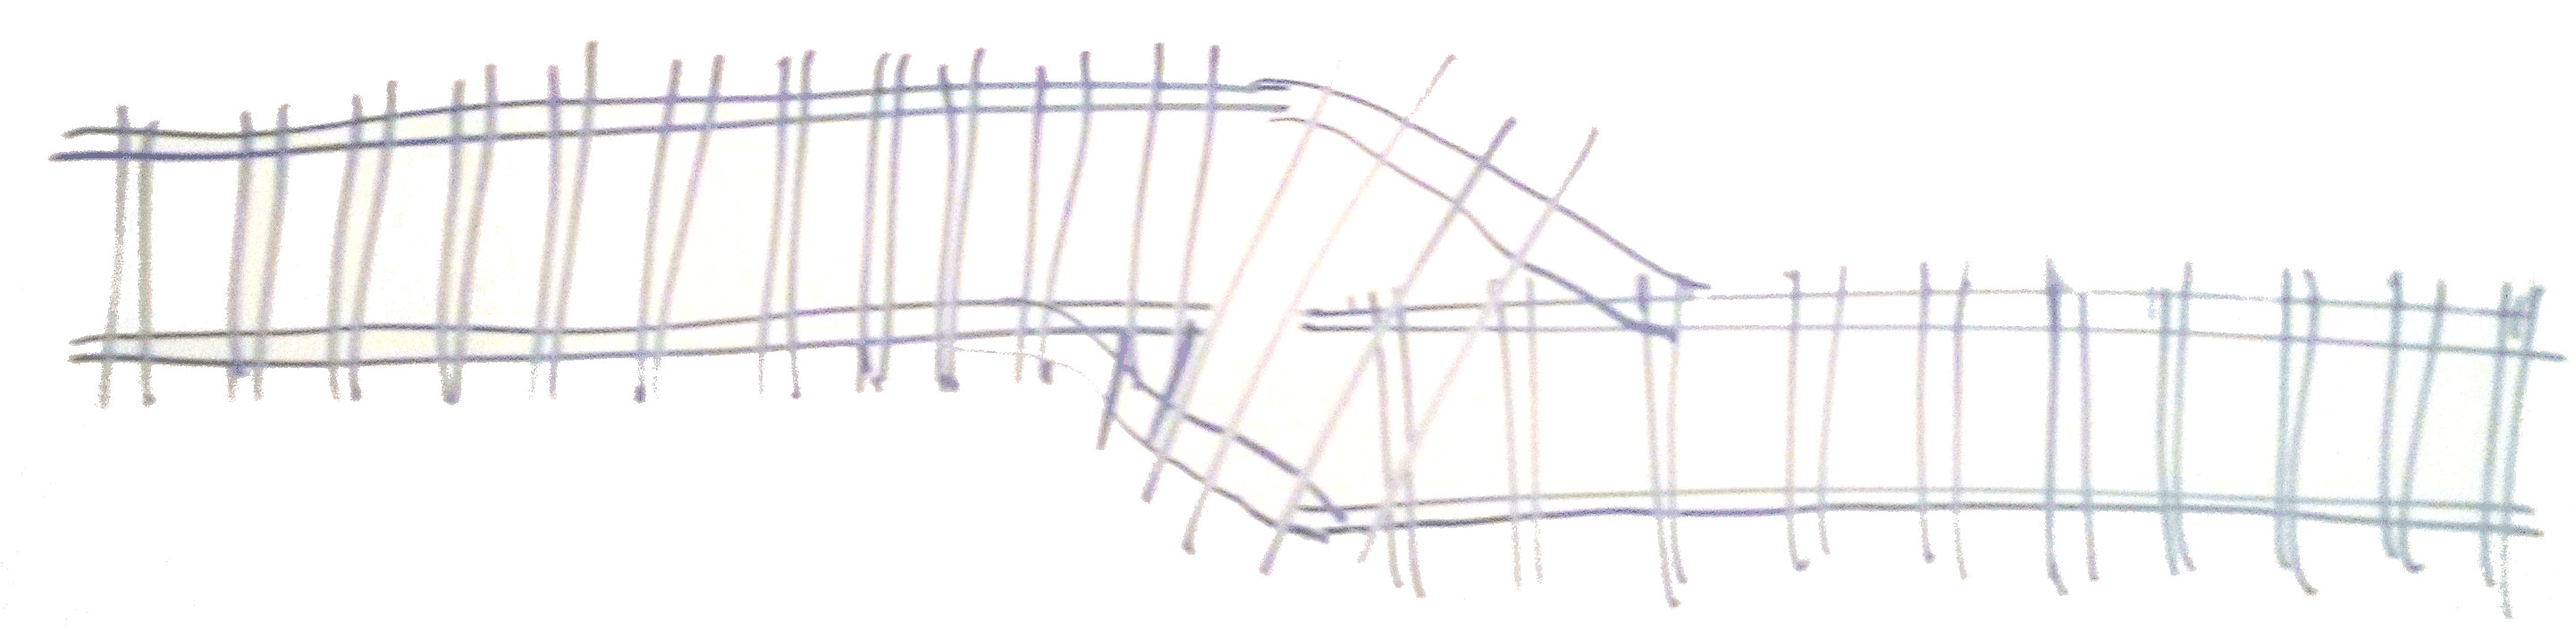
\includegraphics[width=.7\textwidth]{L02/003_patch}
\end{center}

\paragraph{Fault Tolerance.} You are never going to remove all of the
bugs, and some errors arise from conditions beyond your control
(such as hardware faults). It's worthwhile to tolerate faults too.
Strategies include redundancy and isolation. An example of redundancy
is provisioning extra hardware in case a server goes down. Isolation
includes things as simple as checking preconditions.

\begin{center}
  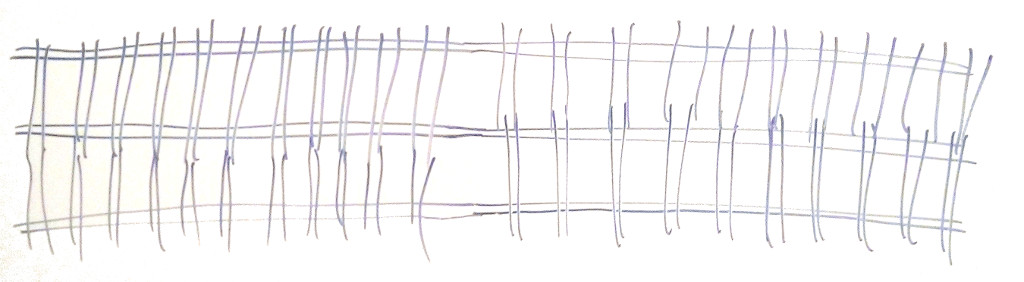
\includegraphics[width=.7\textwidth]{L02/004_fault_tolerance}
\end{center}


\section*{Testing vs Debugging}
Recall from last time:

{\bf Testing}: evaluating software by observing its execution.\\
{\bf Debugging}: finding (and fixing) a fault given a failure.

I said that you really need to automate your tests. But even so,
testing is still hard: only certain inputs expose the fault in the
form of a failure. As you've experienced, debugging is hard too: you
have the failure, but you have to find the fault.

\paragraph{Contrived example.} Consider the following code:
\begin{lstlisting}
  if (x - 100 <= 0)
    if (y - 100 <= 0)
      if (x + y - 200 == 0)
        crash();
\end{lstlisting}
Only one input, {\tt x = 100} and {\tt y = 100}, will trigger the
crash.  If you're just going to do a random brute-force search over
all 32-bit integers, you are never going to find the crash.

\end{document}
